\documentclass[compress]{beamer}

\mode<presentation>
{
\useoutertheme[subsection=false,footline=authorinstitutetitle]{miniframes}
\useinnertheme{rectangles}
\usecolortheme{whale}
\usecolortheme{orchid}
\usefonttheme{professionalfonts}

\setbeamertemplate{footline}
{
	\begin{beamercolorbox}[wd=0.33\textwidth,ht=2.2ex,dp=0.8ex,leftskip=1.4em,rightskip=1.4em]{author in head/foot}% 
		\usebeamerfont{author in head/foot}%
		\insertshortauthor%
	\end{beamercolorbox}%
 	\vspace*{-3.0ex}\hspace*{0.33\textwidth}%
 	\begin{beamercolorbox}[wd=0.33\textwidth,ht=2.2ex,dp=0.8ex,left,leftskip=1.4em,rightskip=1.4em]{author in head/foot}% 
     	\usebeamerfont{institute in head/foot}%
 		\insertshortinstitute%
 	\end{beamercolorbox}%
  	\begin{beamercolorbox}[wd=0.34\textwidth,ht=2.2ex,dp=0.8ex,left,leftskip=1.4em,rightskip=1.4em]{title in head/foot}
      	\usebeamerfont{title in head/foot}
  		\insertshorttitle
  		\hfill\insertframenumber\,/\,\inserttotalframenumber
  	\end{beamercolorbox}
}

\beamertemplatenavigationsymbolsempty
\setbeamercovered{transparent}

}


\usepackage[ngerman]{babel}
\usepackage[utf8]{inputenc}

% font definitions, try \usepackage{ae} instead of the following
% three lines if you don't like this look
\usepackage{mathpazo}
\usepackage[scaled=.90]{helvet}
%\usepackage{helvet}
\usepackage{courier}
\usepackage{graphics}
\usepackage{amsmath}
\usepackage{amsfonts}
\usepackage{amssymb}


\usepackage[T1]{fontenc}
\usepackage{multicol}
\usepackage{verbatim}
\usepackage{listings}
\usepackage{xcolor}

\newcommand{\textqt}[1]{\frqq #1\flqq\ }


\hypersetup{
   pdftitle={Seminarvortrag},
   colorlinks=false,
   linkcolor=black,
   pdfpagemode=None,
   pdfstartview=Fit
  }

\author[Pfann]{%
  Johannes Pfann
}


\date{}

\institute[FAU Erlangen-Nürnberg]{
  Lehrstuhl für Software Engineering\\
  Friedrich-Alexander-Universität Erlangen-Nürnberg
}

\subject{Seminar Design Patterns und Anti-Patterns}
\title{Vortragsthema}

\newcommand{\changefont}[3]{
\fontfamily{#1}\fontseries{#2}\fontshape{#3}\selectfont}

\lstnewenvironment{beispiel}[3]{
    \lstset{language=#1, 
    numberbychapter=true,
    basicstyle=\ttfamily\small, 
    identifierstyle=\color{black}, 
    keywordstyle=\color{blue}, 
    stringstyle=\color{verde}, 
    commentstyle=\color{red}, 
   	breaklines=true, 
   	numbers=left,
   	label=#2,
   	caption=#3,
   	numberstyle=\small, 
   	frame=single}
   	\begingroup
   	\nopagebreak
   	}
   	{\endgroup}%  	   
   	


\AtBeginSection[]
{
  \begin{frame}
    \frametitle{Gliederung}
    \tableofcontents[currentsection, hideothersubsections]
  \end{frame}
}

\definecolor{dkgreen}{rgb}{0,0.6,0}
\definecolor{gray}{rgb}{0.5,0.5,0.5}
\definecolor{mauve}{rgb}{0.58,0,0.82}

\usepackage[section]{minted}
\definecolor{mintedbackground}{rgb}{0.95,0.95,0.95}

\newmintedfile[javacode]{java}{
	bgcolor=mintedbackground,
	linenos=true,
	numberblanklines=true,
	numbersep=5pt,
	gobble=0,
	funcnamehighlighting=true,
	tabsize=4,
	obeytabs=false,
	mathescape=false
	samepage=true,
	showspaces=false,
	showtabs =false,
	texcl=false,
	breaklines=true,
	fontsize=\scriptsize,
	style=trac
}


\begin{document}


\frame{\titlepage} 

\begin{frame}
	\frametitle{Gliederung}
	\tableofcontents[hideallsubsections]
\end{frame}


\section[Verhaltensmuster]{Verhaltensmuster}

\subsection*{Erzeugungsmuster - Was ist das?}
\begin{frame}
	\frametitle{Verhaltensmuster -- Was ist das?}
	\begin{block}{Verhaltensmuster ...}
	\begin{itemize}
		\item Zuweisung von Zuständigkeiten
		\item Wechselseitige Kommunikation zwischen Objekten
		\item Beschreibung von komplexen Programmabläufen
	\end{itemize}
	\end{block}	
	\begin{block}{Konsequenzen}
	\begin{itemize}
		\item Trennung von Verantwortlichkeiten
		\item Veringerung der Kopplung 
		\item Erhöhung der Flexibilität der Software hinsichtlich ihres Verhaltens
		\item Bessere Verständlichkeit eines Programmablaufes
	\end{itemize}
	\end{block}	
\end{frame}

\subsection*{Typen von Erzeugungsmustern}
\begin{frame}
	\frametitle{Typen von Erzeugungsmustern}
	\begin{block}{Klassenbasiert}
		Klassenbasierte Verhaltensmuster wenden für die VErhaltenszuordnung zu den Klassen das Vererbungsprinzip an. 
		\begin{itemize}
			\item Template Method
			\item Interpreter
		\end{itemize} 	
	\end{block}

	
\end{frame}

\begin{frame}
	\frametitle{Typen von Erzeugungsmustern}
	\begin{block}{Objektbasiert}
		Bei objektbasierten Mustern wird der Erzeugungsprozess an andere Objekte delegiert
				\begin{itemize}
					\item \alert<1-> {Observer}
					\item \alert<1-> {Command}
					\item \alert<1-> {Visitor}
					\item Strategy			
					\item Mediator
					\item Iterator
					\item Memento 
					\item State
					\item Chain of Responsibility
				\end{itemize}	
	\end{block}
\end{frame}


\section[Observer]{Observer}

\subsection{Definition}
\begin{frame}
  \frametitle{Definition}

  \begin{block}{Zweck}
  	Definition einer 1-zu-n-Abhängigkeit zwischen Objekten, damit im Fall einer Zustandsänderung eines Ojbekts alle davon abhängigen Objekte entsprechend benachrichtigt und automatisch aktualisiert werden.
  \end{block}
  	
  \begin{block}{Motivation/Ziel}
  	\begin{itemize}
  		\item asdf
  		\item asdf
  	\end{itemize}
  \end{block}
\end{frame}

\subsection{Klassendiagramm - Observer Pattern}
\begin{frame}
	\frametitle{Observer Pattern}
	\begin{itemize}
		\item Basiert auf Rollen
		\item Stellt Mechanismus zur Broadcast-Kommunikation dar
	\end{itemize}	
	
  	\begin{figure}
		\includegraphics[scale=.4]{paper/observer/observer}
	\end{figure}
\end{frame}


\subsection{Beispiel - Arbeitsvermittlung}
\begin{frame}
	\frametitle{Arbeitsvermittlung}
	\begin{itemize}
		\item 1-zu-n-Kommunikation zwischen Vermittlung und Klienten (Broadcast)
		\item Arbeitsvermittlung kennt weder Anzahl noch konkrete Klienten
		\item Klienten melden sich nur an, wenn sie daran interessiert sind.
	\end{itemize}		 
  	\begin{figure}
		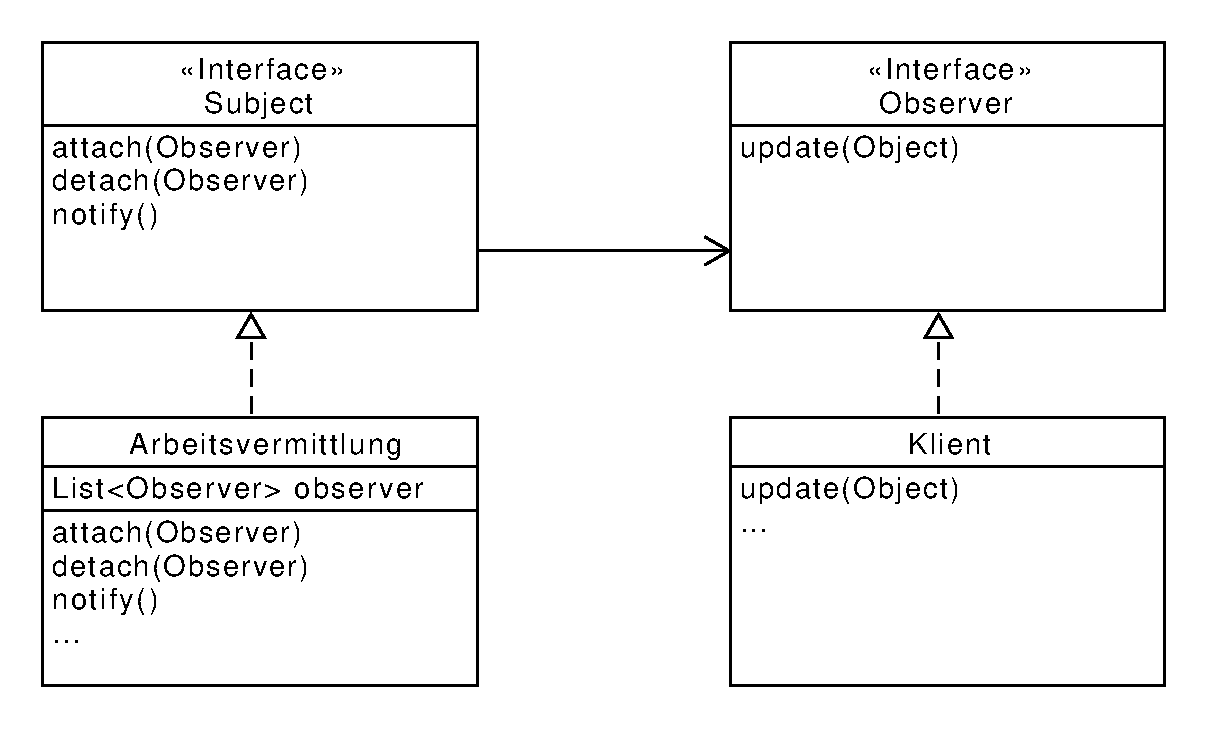
\includegraphics[scale=.4]{paper/observer/arbeitsvermittlung}
	\end{figure}
\end{frame}


\begin{frame}
\frametitle{Beispiel - Klient}
		\javacode{resources/observer_Subject_Interface.java} 
  		\javacode{resources/observer_Klient.java}	  
\end{frame}

\begin{frame}
\frametitle{Beispiel - Arbeitsvermittlung}
		\javacode{resources/observer_Observer_Interface.java}
  		\javacode{resources/observer_Arbeitsvermittlung.java}	  
\end{frame}

\subsection{Implementierungsmöglichkeiten}
\begin{frame}
\frametitle{Implementierungsmöglichkeiten}
		\begin{block}{Push Modell}
		  \begin{itemize}
		  	\item Daten nur in der update-Methode
		  	\item Zugriff auf Subject nicht erlaubt
		  	\item Subjekt muss Interesse der Observer kennen.
		  \end{itemize}
  		\end{block}
  		\begin{block}{Pull Modell}
  		 \begin{itemize}
		  	\item update-Methode ohne Parameter
		  	\item Zugriff auf Subjekt erwünscht
		  	\item Observer müssen Subject kennen
		  \end{itemize}  
  		\end{block}
  		Beides kann auch gemischt weden!
\end{frame}


\begin{frame}
\frametitle{Implementierungsmöglichkeiten}
		  \begin{block}{Observer beobachten mehrere Subects}
		  	\begin{itemize}
		  		\item Observer registriert sich bei mehreren Subjects
		  		\item Muss allerdings unterschiedlich darauf reagieren
		  		\item Lösung: erweiterung der update-Methode mit Subject
		  	\end{itemize}
		  \end{block}
		\javacode{resources/observer_erweiterung_update.java}  		
\end{frame}

\begin{frame}
\frametitle{Implementierungsmöglichkeiten}
		\begin{block}{Ausführung der Updates durch Subject}
  		 \begin{itemize}
		  	\item Weniger fehleranfällig
		  	\item Jedoch zu häufige Updates
		  \end{itemize}  
  		\end{block}		
  		\begin{block}{Ausführung der Updates durch Client}
		  \begin{itemize}
		  	\item Fehleranfälliger
		  	\item Regulierung der Updates
		  \end{itemize}
  		\end{block}
			
\end{frame}


\section[Command]{Command}


\section[Visitor]{Visitor}



\section[Zusammenfassung]{Zusammenfassung}



\section[Quellen]{Quellen}



\end{document}

